\documentclass[10pt]{article}

\usepackage[a4paper,margin=0.65in]{geometry}
\usepackage{amsmath,amssymb}
\usepackage{graphicx}
\usepackage{booktabs}
\usepackage{array}
\usepackage{float}
\usepackage{hyperref}
\usepackage{enumitem}
\usepackage{xcolor}
\usepackage{tikz}
\usetikzlibrary{positioning,arrows.meta,shapes.geometric}

\setlist{nosep,leftmargin=*}
\renewcommand{\arraystretch}{1.2}
\setlength{\parindent}{0pt}
\setlength{\parskip}{2pt}

\tikzset{
layer/.style={
draw,
rounded corners,
minimum width=1.5cm,
minimum height=0.6cm,
align=center,
fill=blue!10,
font=\scriptsize
},
arrow/.style={
-{Latex[length=2mm]},
thin
}
}

\begin{document}

%%%%%%%%%%%%%%%%%%%%%%%%%%%%%%%%%%%%%%%%%%%%%%%%%%%%%%%%%%%%
% TITLE
%%%%%%%%%%%%%%%%%%%%%%%%%%%%%%%%%%%%%%%%%%%%%%%%%%%%%%%%%%%%

\begin{center}

{\large\textbf{Shiv Nadar University Chennai}}

\vspace{2mm}

{\normalsize\textbf{CS3807 -- Deep Learning Laboratory}}

\vspace{2mm}

{\large\textbf{Experiment 5}}

\vspace{1mm}

{\normalsize\textbf{Comprehensive Study of CNN Training, Regularization,}}

{\normalsize\textbf{Optimization, Hyperparameter Tuning, Transfer Learning}}

{\normalsize\textbf{and Cross-Validation}}

\end{center}

\vspace{3mm}

\begin{tabular}{|p{3.4cm}|p{9.0cm}|p{1.4cm}|}
\hline
Degree \& Branch &
B.Tech Artificial Intelligence \& Data Science &
Semester V\\
\hline
Subject Code \& Name &
CS3807 -- Deep Learning Laboratory &
AY: 2026--27\\
\hline
Name & Madhav.S & \\
\hline
Section & AIDS `B' & \\
\hline
Register Number & 24011101066 & \\
\hline
\end{tabular}

%%%%%%%%%%%%%%%%%%%%%%%%%%%%%%%%%%%%%%%%%%%%%%%%%%%%%%%%%%%%
\section*{1. Objective}

The objective of this experiment is to systematically study the effect of
weight initialization, regularization, optimization algorithms, CNN
hyperparameters, transfer learning, fine-tuning and cross-validation on
image classification performance.

A single CNN architecture, MobileNetV2, was used throughout on the
Oxford-IIIT Pet dataset. Each design choice was analyzed using
training/validation curves, and a final configuration was selected
using 5-fold cross-validation and evaluated once on an independent
test set.

%%%%%%%%%%%%%%%%%%%%%%%%%%%%%%%%%%%%%%%%%%%%%%%%%%%%%%%%%%%%
\section*{2. Learning Outcomes}

After completing this experiment, students will be able to:

\begin{itemize}
\item explain different weight initialization strategies;
\item identify and analyze overfitting using training and validation curves;
\item compare SGD, Momentum, RMSProp and Adam;
\item explain CNN hyperparameters such as kernel size, stride, padding and pooling;
\item understand Batch Normalization and Dropout;
\item perform transfer learning and fine-tuning using MobileNetV2;
\item tune important training hyperparameters;
\item apply 5-fold cross-validation for model selection; and
\item justify the final model using accuracy, variability and computational cost.
\end{itemize}

%%%%%%%%%%%%%%%%%%%%%%%%%%%%%%%%%%%%%%%%%%%%%%%%%%%%%%%%%%%%
\section*{3. Dataset and Experimental Setup}

\textbf{Dataset: Oxford-IIIT Pet Dataset}

The Oxford-IIIT Pet Dataset contains 7{,}349 RGB images spanning 37 cat
and dog breeds, loaded directly via \texttt{tensorflow\_datasets}. Every
image was resized to

\[
224\times224\times3
\]

and normalized using MobileNetV2's own \texttt{preprocess\_input}
function, matching the ImageNet statistics the pretrained base expects.

\textbf{Split.} The 7{,}349 images were stratified by breed into a
70/15/15 train/validation/test split:

\begin{center}
\begin{tabular}{|l|c|}
\hline
Split & Number of Images\\
\hline
Training & 5{,}144\\
Validation & 1{,}102\\
Test & 1{,}103\\
\hline
\end{tabular}
\end{center}

The test set was kept completely untouched until Section 8 (Final
Model Evaluation) -- every earlier section, including the 5-fold
cross-validation in Section 7, used only the training split.

%%%%%%%%%%%%%%%%%%%%%%%%%%%%%%%%%%%%%%%%%%%%%%%%%%%%%%%%%%%%
\section*{4. MobileNetV2 Architecture}

MobileNetV2 is a lightweight CNN architecture designed to reduce
computational complexity while maintaining good image representation.

Its important components include:

\begin{itemize}
\item depthwise convolution;
\item pointwise $1\times1$ convolution;
\item inverted residual blocks;
\item linear bottlenecks;
\item batch normalization; and
\item ReLU6 activation.
\end{itemize}

A simplified representation is:

\begin{center}
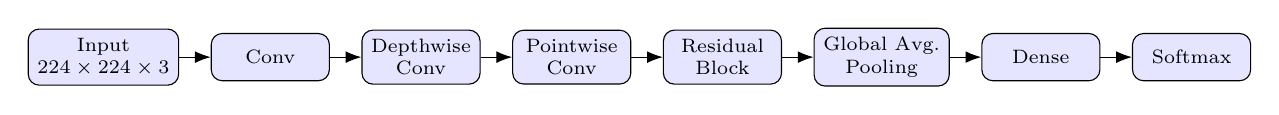
\begin{tikzpicture}[node distance=4mm]

\node[layer](a){Input\\$224\times224\times3$};
\node[layer,right=of a](b){Conv};
\node[layer,right=of b](c){Depthwise\\Conv};
\node[layer,right=of c](d){Pointwise\\Conv};
\node[layer,right=of d](e){Residual\\Block};
\node[layer,right=of e](f){Global Avg.\\Pooling};
\node[layer,right=of f](g){Dense};
\node[layer,right=of g](h){Softmax};

\foreach \x/\y in {a/b,b/c,c/d,d/e,e/f,f/g,g/h}
\draw[arrow](\x)--(\y);

\end{tikzpicture}
\end{center}

\textbf{Note:} The above diagram is a simplified conceptual representation
rather than the complete MobileNetV2 architecture. In this experiment,
the pretrained ImageNet base is followed by GlobalAveragePooling2D,
an optional BatchNormalization layer, a Dense(128, ReLU) layer, an
optional Dropout layer, and a final Dense(37, softmax) layer.

%%%%%%%%%%%%%%%%%%%%%%%%%%%%%%%%%%%%%%%%%%%%%%%%%%%%%%%%%%%%
\section*{5. Weight Initialization}

Four initialization strategies were compared for the newly-added
classifier head (the pretrained convolutional base stayed frozen and
retained its own ImageNet weights): Zero, Random (Normal), Xavier/Glorot
and He, each trained for 8 epochs with Adam.

\begin{center}
\includegraphics[width=0.72\linewidth]{plot01_training_loss_vs_epoch_initialization.pdf}
\end{center}

\textbf{Inference:} Zero initialization never leaves loss $\approx3.61$
because every head neuron receives an identical gradient and stays
perfectly symmetric -- the network cannot break symmetry on its own.
Random, Xavier and He all fall from around 1.2--1.4 to under 0.2 within
a couple of epochs, confirming that any asymmetric initialization is
enough for this frozen-base setup to learn.

\begin{center}
\includegraphics[width=0.72\linewidth]{plot02_val_accuracy_vs_epoch_initialization.pdf}
\end{center}

\textbf{Inference:} Zero initialization is stuck at $2.7\%$ (random
guessing among 37 classes), while Random, Xavier and He all climb
past $90\%$ validation accuracy. He initialization edges ahead
slightly, peaking at $92.11\%$, with Xavier close behind at $91.74\%$ --
a small but expected gain, since He initialization is designed for the
ReLU activation used in the classifier head.

%%%%%%%%%%%%%%%%%%%%%%%%%%%%%%%%%%%%%%%%%%%%%%%%%%%%%%%%%%%%
\section*{6. Regularization and Overfitting}

Four settings were compared for 10 epochs each: no regularization,
L2 regularization ($\lambda=10^{-3}$), Dropout (rate 0.5), and Batch
Normalization on the head.

\begin{center}
\includegraphics[width=0.85\linewidth]{plot03_train_val_accuracy_vs_epoch_regularization.pdf}
\end{center}

\textbf{Inference:} With no regularization, training accuracy shoots
past $99\%$ by epoch 5 while validation accuracy plateaus around
$91$--$92\%$ -- a clear, widening generalization gap. Dropout and L2
keep training accuracy lower for longer, and Batch Normalization
converges fastest of all (training accuracy above $98\%$ by epoch 4)
.

\begin{center}
\includegraphics[width=0.85\linewidth]{plot04_train_val_loss_vs_epoch_regularization.pdf}
\end{center}

\textbf{Inference:} Training loss keeps falling in every configuration,
but validation loss for ``No Regularization'' and ``Batch
Normalization'' starts creeping back up after epoch 5--6 even as
training loss keeps dropping. This shows overfitting.
L2's loss values sit visibly higher throughout, simply because the
penalty term is added directly into the plotted loss, not because the
model fits worse.

%%%%%%%%%%%%%%%%%%%%%%%%%%%%%%%%%%%%%%%%%%%%%%%%%%%%%%%%%%%%
\section*{7. Batch Normalization}

Batch Normalization normalizes activations within a mini-batch during
training.

For a mini-batch

\[
x_1,x_2,\ldots,x_m,
\]

the batch mean is

\[
\mu_B=\frac{1}{m}\sum_{i=1}^{m}x_i
\]

and the batch variance is

\[
\sigma_B^2=
\frac{1}{m}\sum_{i=1}^{m}(x_i-\mu_B)^2.
\]

The normalized activation is

\[
\hat{x}_i=
\frac{x_i-\mu_B}
{\sqrt{\sigma_B^2+\epsilon}}.
\]

The final output is

\[
y_i=\gamma\hat{x}_i+\beta,
\]

where $\gamma$ and $\beta$ are learnable parameters.

\subsection*{Numerical Example}

Consider

\[
x=[2,4,6,8].
\]

The mean is

\[
\mu_B=\frac{2+4+6+8}{4}=5.
\]

The variance is

\[
\sigma_B^2=
\frac{(2-5)^2+(4-5)^2+(6-5)^2+(8-5)^2}{4}
=5.
\]

Therefore,

\[
\sqrt{5}\approx2.236.
\]

Ignoring the very small $\epsilon$,

\[
\hat{x}_1=\frac{2-5}{2.236}\approx-1.342,\quad
\hat{x}_2=\frac{4-5}{2.236}\approx-0.447,
\]
\[
\hat{x}_3=\frac{6-5}{2.236}\approx0.447,\quad
\hat{x}_4=\frac{8-5}{2.236}\approx1.342.
\]

Hence,

\[
\boxed{
\hat{x}\approx[-1.342,-0.447,0.447,1.342]
}
\]

If $\gamma=1$ and $\beta=0$, these are the final outputs.

\textbf{Inference:} Batch Normalization produces approximately
zero-centred and unit-scaled activations for this mini-batch. The
learnable $\gamma$ and $\beta$ allow the network to learn an appropriate
scale and shift instead of being forced to keep every activation
standardized.

\begin{center}
\includegraphics[width=0.72\linewidth]{plot05_with_vs_without_bn.pdf}
\end{center}

\textbf{Inference:} With BN peaks at $92.01\%$ (epoch 7) and Without BN
peaks slightly higher at $92.29\%$ (epoch 8) -- BN sped up training
accuracy noticeably (past $98\%$ by epoch 4 versus a slower climb
without it) but did not translate into a clearly better validation
accuracy here, most likely because MobileNetV2's frozen convolutional
base is already full of its own internal BatchNorm layers, so adding
one more on top of an already-normalized feature vector has limited
extra benefit.

%%%%%%%%%%%%%%%%%%%%%%%%%%%%%%%%%%%%%%%%%%%%%%%%%%%%%%%%%%%%
\section*{8. Optimization Algorithms}

SGD, Momentum, RMSProp and Adam were compared for 10 epochs each, all
other settings held fixed (Dropout 0.5, BatchNorm on, learning rate
$10^{-3}$).

\begin{center}
\includegraphics[width=0.72\linewidth]{plot06_training_loss_vs_epoch_optimizers.pdf}
\end{center}

\begin{center}
\includegraphics[width=0.72\linewidth]{plot07_val_accuracy_vs_epoch_optimizers.pdf}
\end{center}

\begin{center}
\begin{tabular}{|l|c|c|c|c|}
\hline
Optimizer & Final Loss & Best Val. Accuracy & Epoch to Converge & Time\\
\hline
SGD & 1.2980 & 81.31\% & 10 & 74.6 s\\
Momentum & 0.3619 & 91.38\% & 5 & 74.9 s\\
RMSProp & \textbf{0.1765} & \textbf{92.38\%} & 7 & 74.7 s\\
Adam & \textbf{0.1379} & 91.74\% & 9 & 75.0 s\\
\hline
\end{tabular}
\end{center}

\textbf{Inference:} Plain SGD is still climbing at epoch 10 and lands
over 10 points behind every adaptive method -- with no momentum term,
a $10^{-3}$ learning rate is simply too small to move quickly through
this loss surface. RMSProp reaches the best validation accuracy
($92.38\%$) fastest of the three adaptive methods, while Adam achieves
the lowest final training loss; both clearly outperform Momentum and
SGD within the same 10-epoch, 75-second training budget.

%%%%%%%%%%%%%%%%%%%%%%%%%%%%%%%%%%%%%%%%%%%%%%%%%%%%%%%%%%%%
\section*{9. CNN Hyperparameter Tuning}

Learning rate, batch size and dropout rate were each swept
independently (6 epochs, one hyperparameter changed at a time, all
others fixed at LR $=10^{-3}$, batch size 32, dropout 0.25):

\begin{center}
\begin{tabular}{|l|l|l|}
\hline
Hyperparameter & Values Tested & Result (Best Val. Accuracy)\\
\hline
Learning Rate & $0.001,\;0.0001$ & $0.001\to92.47\%$; $0.0001\to90.20\%$\\
Batch Size & 16, 32, 64 & $16\to91.02\%$; $32\to91.47\%$; $64\to91.38\%$\\
Dropout Rate & 0, 0.25, 0.5 & $0\to91.38\%$; $0.25\to91.56\%$; $0.5\to91.83\%$\\
\hline
\end{tabular}
\end{center}

Optimizer choice (Section 8) and the frozen-base vs.\ fine-tuning
trade-off (Section 10) were investigated separately, since both
already required their own dedicated comparisons above.

For CNN concepts, the following were also reviewed: kernel/filter,
stride, padding, pooling, number of channels, and depthwise separable
convolution. For a convolution operation, the output dimension is

\[
O=
\left\lfloor
\frac{N+2P-K}{S}
\right\rfloor+1,
\]

where $N$ is input size, $K$ is kernel size, $P$ is padding and $S$ is
stride. For example, $N{=}224,K{=}3,P{=}1,S{=}1$ gives $O=224$
(same-padding, size-preserving), while $N{=}224,K{=}3,P{=}0,S{=}2$
gives $O=111$ (a strided, downsampling convolution).

\begin{center}
\includegraphics[width=0.48\linewidth]{plot08_lr_vs_val_accuracy.pdf}
\hfill
\includegraphics[width=0.48\linewidth]{plot09_batchsize_vs_val_accuracy.pdf}
\end{center}

\begin{center}
\includegraphics[width=0.55\linewidth]{plot10_dropout_vs_val_accuracy.pdf}
\end{center}

\textbf{Inference:} The higher learning rate ($10^{-3}$) beats the
lower one by over 2 points within this short 6-epoch -- $10^{-4}$
simply hasn't taken enough steps yet. Batch size 32 is a mild sweet
spot between 16 and 64, and accuracy rises steadily with more dropout
(0 to 0.5), suggesting the classifier head is prone to overfitting
quickly and benefits from stronger regularization even in this short
run.

%%%%%%%%%%%%%%%%%%%%%%%%%%%%%%%%%%%%%%%%%%%%%%%%%%%%%%%%%%%%
\section*{10. Transfer Learning and Fine-Tuning}

MobileNetV2 pretrained on ImageNet was used for both cases below.

\subsection*{Case A: Feature Extraction}

\[
\text{Pretrained MobileNetV2}
\rightarrow
\text{Freeze Base}
\rightarrow
\text{New Classifier}
\]

The pretrained convolutional layers were frozen and only the newly
added classification head was trained for 8 epochs.

\subsection*{Case B: Fine-Tuning}

\[
\text{Pretrained MobileNetV2}
\rightarrow
\text{Unfreeze Last 30 Layers}
\rightarrow
\text{LR}=10^{-5}
\]

The last 30 layers of the pretrained base were unfrozen and trained
for a further 8 epochs at a much smaller learning rate ($10^{-5}$ vs.\
$10^{-3}$), continuing from the feature-extraction weights.

\begin{center}
\includegraphics[width=0.72\linewidth]{plot11_feature_extraction_vs_finetuning.pdf}
\end{center}

\begin{center}
\includegraphics[width=0.72\linewidth]{plot12_loss_feature_extraction_vs_finetuning.pdf}
\end{center}

\textbf{Inference:} Feature extraction alone already reaches $91.74\%$
validation accuracy by epoch 7, and fine-tuning the last 30 layers
does not push past that peak within its own 8 epochs (settling around
$91.1$--$91.7\%$). With a frozen-base model already this strong,
a longer fine-tuning run or unfreezing more layers
would likely be needed to see a clearer gain.

\textbf{Discussion:} Fine-tuning uses a smaller learning rate than
training a freshly-initialized classifier because the unfrozen layers
already hold well-trained ImageNet weights; a large learning rate
would overwrite those useful features with large, disruptive updates
before the new classifier has had a chance to guide them gently.

%%%%%%%%%%%%%%%%%%%%%%%%%%%%%%%%%%%%%%%%%%%%%%%%%%%%%%%%%%%%
\section*{11. K-Fold Cross-Validation}

Four configurations, chosen based on the results of the sections above,
were evaluated using 5-fold cross-validation on the training split
only (5 epochs per fold):

\begin{center}
\begin{tabular}{|l|c|c|c|c|c|c|}
\hline
Configuration & F1 & F2 & F3 & F4 & F5 & Mean $\pm$ SD\\
\hline
C1: Adam, Dropout 0.5, BN & 91.06 & 91.35 & 91.35 & 91.45 & 90.95 & $91.23\pm0.19$\\
C2: Adam (LR $10^{-4}$), Dropout 0.25, BN & 88.14 & 87.56 & 88.82 & 87.46 & 89.59 & $88.32\pm0.80$\\
\textbf{C3: RMSProp, Dropout 0.5, BN} & \textbf{91.06} & \textbf{91.64} & \textbf{91.74} & \textbf{91.55} & \textbf{91.63} & $\mathbf{91.52\pm0.24}$\\
C4: Adam, L2 $=10^{-3}$, BN & 90.77 & 90.96 & 91.74 & 90.48 & 90.56 & $90.90\pm0.45$\\
\hline
\end{tabular}
\end{center}

\[
\boxed{\bar{A}_{C3}=91.52\%\pm0.24}
\]

\begin{center}
\includegraphics[width=0.72\linewidth]{plot13_5fold_cv_accuracy.pdf}
\end{center}

\textbf{Inference:} C3 (RMSProp, Dropout 0.5, BN) wins on both counts
that matter -- the highest mean accuracy \emph{and} the joint-lowest
standard deviation (tied with C1) -- so it was selected as the final
configuration. C2's low learning rate ($10^{-4}$) clearly needed more
than 5 epochs per fold to catch up, both scoring lowest and varying
most (SD $=0.80$) across folds.

%%%%%%%%%%%%%%%%%%%%%%%%%%%%%%%%%%%%%%%%%%%%%%%%%%%%%%%%%%%%
\section*{12. Final Model Evaluation}

Configuration C3 (RMSProp, Dropout 0.5, Batch Normalization) was
retrained on the complete training split for 12 epochs and evaluated
once on the untouched test set:

\begin{center}
\begin{tabular}{|l|c|}
\hline
Metric & Value\\
\hline
Mean CV Accuracy & 91.52\%\\
CV Standard Deviation & 0.24\\
Test Accuracy & 90.03\%\\
Precision (macro) & 0.9021\\
Recall (macro) & 0.9002\\
F1-score (macro) & 0.8997\\
Training Time & 87.1 s\\
Number of Parameters & 2{,}431{,}845\\
\hline
\end{tabular}
\end{center}

\begin{center}
\includegraphics[width=0.85\linewidth]{plot14_confusion_matrix.pdf}
\end{center}

\textbf{Inference:} Several breeds are classified with perfect
accuracy on the test set (Yorkshire Terrier, Siamese, Sphynx, Great
Pyrenees, Leonberger), while the confusion that does occur is
concentrated in visually similar breed pairs -- Russian Blue vs.\
British Shorthair (grey short-haired cats) and American Pit Bull
Terrier vs.\ Staffordshire Bull Terrier (near-identical short-haired
dog breeds) are the two most frequently confused pairs. 

\begin{center}
\includegraphics[width=0.65\linewidth]{plot15_misclassified_images.pdf}
\end{center}

\textbf{Inference:} The sampled misclassified images mostly show
partial views, unusual poses or lighting, or a genuinely similar-looking
breed being predicted -- consistent with the confusion pairs identified
above rather than any obvious data or labelling problem.

%%%%%%%%%%%%%%%%%%%%%%%%%%%%%%%%%%%%%%%%%%%%%%%%%%%%%%%%%%%%
\section*{13. Overall Results}

\begin{center}
\begin{tabular}{|l|c|c|c|c|}
\hline
Configuration & CV Accuracy & SD & Test/Val. Accuracy & Training Time\\
\hline
Baseline (No Regularization) & -- & -- & 91.56\% (val) & --\\
Best Initialization (He) & -- & -- & 92.11\% (val) & --\\
Best Regularization (Dropout, tied with BN) & -- & -- & 92.01\% (val) & --\\
Best Optimizer (RMSProp) & -- & -- & 92.38\% (val) & 74.7 s\\
Best Hyperparameters (LR $=10^{-3}$) & -- & -- & 92.47\% (val) & --\\
Fine-Tuned Model & -- & -- & 91.74\% (val) & --\\
\textbf{Final Selected Model (C3)} & \textbf{91.52\%} & \textbf{0.24} & \textbf{90.03\% (test)} & \textbf{87.1 s}\\
\hline
\end{tabular}
\end{center}

The individual studies (initialization, regularization,
optimizer, hyperparameters, fine-tuning) each report the best
\emph{validation} accuracy from their own single run, since only the
final, cross-validated configuration was retrained and evaluated on
the held-out test set. The final model's test accuracy is $90.03\%$.  C3 was selected over the
individually-higher-scoring ablation runs above because it was the
only configuration validated for both accuracy \emph{and}
consistency (low standard deviation) across five independent folds,
rather than a single train/validation split.

%%%%%%%%%%%%%%%%%%%%%%%%%%%%%%%%%%%%%%%%%%%%%%%%%%%%%%%%%%%%
\section*{14. Discussion Questions}

\begin{enumerate}
\item \textbf{What is the difference between model parameters and hyperparameters?}
Parameters (weights, biases) are learned automatically during training via
backpropagation. Hyperparameters (learning rate, batch size, dropout
rate, number of layers) are set by the practitioner before training
and control how that learning happens.

\item \textbf{Why is weight initialization important?}
It determines the starting point of optimization. A poor starting
point can cause vanishing/exploding activations or, in the worst case
(zero initialization), prevent the network from learning at all.

\item \textbf{Why can zero initialization be problematic for neural networks?}
Every neuron in a layer receives the same input and the same gradient,
so they all update identically forever -- the network stays perfectly
symmetric and effectively behaves like a single neuron per layer, as
seen directly in Section 5 (stuck at $2.7\%$ accuracy).

\item \textbf{Compare Xavier and He initialization.}
Both keep the variance of activations stable across layers, but Xavier
assumes a linear/tanh-like activation while He accounts for ReLU
zeroing out roughly half the activations, using a variance scaled by
$2/n$ instead of $1/n$. He is generally preferred for ReLU networks,
matching its slightly better result here ($92.11\%$ vs.\ $91.74\%$).

\item \textbf{How can training and validation curves be used to identify overfitting?}
Overfitting is visible when training accuracy keeps rising (or training
loss keeps falling) while validation accuracy plateaus or validation
loss starts rising -- exactly what appeared for the ``No Regularization''
configuration in Section 6.

\item \textbf{How does Dropout reduce overfitting?}
By randomly zeroing a fraction of neurons on each training step, it
prevents co-adaptation between neurons and forces the network to learn
more redundant, robust features rather than memorizing the training
set.

\item \textbf{What is the purpose of Batch Normalization?}
It normalizes layer activations within each mini-batch, stabilizing
and speeding up training, reducing sensitivity to initialization, and
providing a mild regularizing effect.

\item \textbf{Explain the numerical Batch Normalization example.}
For $x=[2,4,6,8]$, the mean is 5 and variance is 5, giving normalized
values $\approx[-1.342,-0.447,0.447,1.342]$ -- centred at zero with unit
variance, exactly as Section 7 works out step by step.

\item \textbf{What are the roles of $\gamma$ and $\beta$?}
They let the network undo the normalization if that is what's optimal
-- $\gamma$ rescales and $\beta$ re-shifts the normalized activations,
so BatchNorm never strictly limits what the layer can represent.

\item \textbf{Compare SGD, Momentum, RMSProp and Adam.}
SGD is the simplest and slowest to converge, as seen in Section 8
(still at $81.31\%$ after 10 epochs). Momentum accelerates it using
past gradients. RMSProp and Adam both use per-parameter adaptive
learning rates, converging fastest and most reliably here
($92.38\%$ and $91.74\%$ respectively).

\item \textbf{What happens when the learning rate is too large?}
Updates overshoot the minimum, and loss can oscillate or diverge
instead of decreasing steadily.

\item \textbf{What happens when the learning rate is too small?}
Training becomes very slow to converge, as seen with LR $=10^{-4}$ in
Section 9, which still trailed the $10^{-3}$ run by over 2 points
after the same number of epochs.

\item \textbf{What is the effect of increasing batch size?}
Gradient estimates become less noisy (more stable updates) but there
are fewer updates per epoch; very large batches can also generalize
slightly worse, matching batch size 64 scoring marginally below 32 in
Section 9.

\item \textbf{Explain stride and padding.}
Stride is the step size the convolution kernel moves across the input;
larger strides downsample the output. Padding adds extra pixels
(typically zeros) around the input border, letting the output size be
controlled independently of the kernel size (e.g.\ ``same'' padding
keeps the spatial size unchanged).

\item \textbf{Why is MobileNetV2 computationally efficient?}
It replaces standard convolutions with depthwise separable
convolutions (a depthwise pass followed by a $1\times1$ pointwise
pass), which need far fewer multiply-accumulate operations for a
similar receptive field.

\item \textbf{What is depthwise separable convolution?}
A standard convolution factored into two cheaper steps: a depthwise
convolution that filters each input channel independently, followed by
a $1\times1$ pointwise convolution that combines the channels.

\item \textbf{What is transfer learning?}
Reusing a model already trained on a large dataset (ImageNet) as the
starting point for a new, smaller task -- implemented here for the
Oxford-IIIT Pet dataset via MobileNetV2.

\item \textbf{Differentiate feature extraction and fine-tuning.}
Feature extraction keeps the entire pretrained base frozen and only
trains the new classifier head. Fine-tuning additionally unfreezes
some of the base's later layers and trains them (at a small learning
rate) so they adapt to the new dataset.

\item \textbf{Why is a smaller learning rate generally used during fine-tuning?}
The unfrozen layers already hold useful pretrained weights; a large
learning rate would apply large, disruptive updates that overwrite
those features before the classifier can guide them usefully.

\item \textbf{Why is K-Fold Cross-Validation useful for hyperparameter selection?}
It evaluates a configuration across several different train/validation
splits instead of just one, giving both a more reliable accuracy
estimate and a measure of how much that estimate varies (Section 11).

\item \textbf{Why must the test set remain untouched during tuning?}
If the test set influences any decision (choice of hyperparameters,
architecture, or model), it stops being an independent measure of
generalization and the reported accuracy becomes optimistically
biased.

\item \textbf{Why should mean and standard deviation both be reported?}
Mean accuracy alone hides how consistent a configuration is; two
configurations with the same mean can have very different reliability,
as seen between C1 (SD $0.19$) and C4 (SD $0.45$) in Section 11.

\item \textbf{Is the highest validation accuracy always sufficient to select a model?}
No -- a single high validation score can come from a lucky split. C3
was chosen here not for having the single highest number anywhere in
the notebook, but for combining a high \emph{mean} with a low standard
deviation across five independent folds.
\end{enumerate}

%%%%%%%%%%%%%%%%%%%%%%%%%%%%%%%%%%%%%%%%%%%%%%%%%%%%%%%%%%%%
\section*{15. Additional Exercise: New Configurations via 5-Fold Cross-Validation}

Two new combinations of learning rate, dropout, batch size and
fine-tuning strategy were evaluated with 5-fold cross-validation and
compared against the previously selected configuration, C3:

\begin{center}
\small
\begin{tabular}{|p{5.2cm}|c|c|c|c|c|c|}
\hline
Configuration & F1 & F2 & F3 & F4 & F5 & Mean $\pm$ SD\\
\hline
N1: LR $10^{-4}$, Dropout 0.5, Batch 16, Fine-Tuned & 89.60 & 90.96 & 89.70 & 87.95 & 89.40 & $89.52\pm0.96$\\
N2: LR $10^{-3}$, Dropout 0.1, Batch 64, Feature-Extraction & 89.70 & 91.45 & 91.55 & 89.50 & 90.76 & $90.59\pm0.85$\\
\textbf{C3 (previous best, for comparison)} & \textbf{91.06} & \textbf{91.64} & \textbf{91.74} & \textbf{91.55} & \textbf{91.63} & $\mathbf{91.52\pm0.24}$\\
\hline
\end{tabular}
\normalsize
\end{center}

\textbf{Inference:} Neither new configuration beats C3 on mean accuracy
or consistency. N1 combines a low learning rate with fine-tuning, but
its short 3-epoch fine-tuning phase and small batch size leave it both
the lowest-scoring and the most variable (SD $=0.96$) of the three. N2
does better without any fine-tuning at all, suggesting the higher
learning rate and larger batch size are more responsible for its
improvement over N1 than the frozen-vs-fine-tuned choice is.

%%%%%%%%%%%%%%%%%%%%%%%%%%%%%%%%%%%%%%%%%%%%%%%%%%%%%%%%%%%%
\section*{16. Conclusion}

\begin{itemize}
\item Compared four weight initialization schemes on a frozen MobileNetV2
classifier head: Zero initialization failed completely ($2.7\%$,
random-guess level), while Random, Xavier and He all converged
normally, with He slightly ahead at $92.11\%$.
\item Demonstrated overfitting directly: an unregularized head reached
$99.8\%$ training accuracy while validation accuracy plateaued near
$91$--$92\%$; Dropout and Batch Normalization both curbed this gap.
\item Compared SGD, Momentum, RMSProp and Adam under identical
conditions -- RMSProp reached the best validation accuracy
($92.38\%$), with plain SGD trailing by over 10 points in the same
10-epoch budget.
\item Swept learning rate, batch size and dropout rate independently,
finding LR $=10^{-3}$, batch size 32, and dropout 0.5 each performed
best within their own sweep.
\item Implemented both feature extraction and fine-tuning on
MobileNetV2; fine-tuning the last 30 layers did not clearly improve on
feature extraction's $91.74\%$ peak within an 8-epoch budget.
\item Selected a final configuration (RMSProp, Dropout 0.5, Batch
Normalization) using 5-fold cross-validation on four candidates
($91.52\%\pm0.24$, the best mean \emph{and} joint-lowest variability),
then evaluated it once on a completely untouched test set, reaching
$90.03\%$ test accuracy with a macro F1-score of $0.8997$.
\item Two additional hyperparameter combinations were tested via
5-fold CV and both fell short of the selected configuration, confirming
it as the preferred choice.
\end{itemize}

%%%%%%%%%%%%%%%%%%%%%%%%%%%%%%%%%%%%%%%%%%%%%%%%%%%%%%%%%%%%
\section*{17. Source Code}

The complete implementation, exactly as run on Kaggle, is hosted on GitHub.

\url{https://github.com/smadhav2024/Deep_Learning_Lab/tree/main/Lab%205}

%%%%%%%%%%%%%%%%%%%%%%%%%%%%%%%%%%%%%%%%%%%%%%%%%%%%%%%%%%%%
\section*{18. References}

\begin{enumerate}
\item Ian Goodfellow, Yoshua Bengio and Aaron Courville,
\emph{Deep Learning}, MIT Press, 2016.

\item Sergey Ioffe and Christian Szegedy,
``Batch Normalization: Accelerating Deep Network Training by Reducing
Internal Covariate Shift,'' ICML, 2015.

\item Mark Sandler, Andrew Howard, Menglong Zhu, Andrey Zhmoginov and
Liang-Chieh Chen, ``MobileNetV2: Inverted Residuals and Linear
Bottlenecks,'' CVPR, 2018.

\item Omkar M. Parkhi, Andrea Vedaldi, Andrew Zisserman and C. V. Jawahar,
``Cats and Dogs,'' IEEE Conference on Computer Vision and Pattern
Recognition, 2012.

\item TensorFlow Documentation:
\url{https://www.tensorflow.org}

\item Keras Documentation:
\url{https://keras.io}
\end{enumerate}

\end{document}
